\documentclass[a4paper,11pt]{article}

\usepackage{amsmath}
\usepackage{amssymb}
\usepackage{amsfonts}
\usepackage{graphicx}
\usepackage{subcaption}
\usepackage{microtype}
\usepackage{algpseudocode, algorithm}
\PassOptionsToPackage{hyphens}{url}\usepackage{hyperref}
\usepackage{physics}
\usepackage{cleveref}

\title{Downsampling inelastic cyclic stress-strain data while preserving its curvature}
\author{A Hartloper}

\begin{document}
\maketitle

\begin{abstract}
    A downsampling algorithm for stress-strain data that uses few points but retains curvature within a pre-defined tolerance is developed in this document.
\end{abstract}

\section{Introduction}

The raw data (i.e., extensometer displacement, load cell force) in experiments used for material model calibration are typically sampled at 10~Hz in the EPFL test setup.
As experiments range from around a few minutes (e.g., LP1) to hours (LP5), this results in thousands to hundreds of thousands of data points for each experiment.
However, the sampled data is often denser than required to reasonably describe the stress-strain behavior of materials under the applied strain rates.
When it comes to calibrating material models, the time required is proportional to the number of data points.
Therefore, time can be saved by reducing the number of data points prior to running the calibration while maintaining the fidelity of the data.

Experience has shown that the fidelity of an experiment can be kept with around 10--100 times less points depending on the load protocol.
Calibrating the UVC model with ten load protocols \emph{without} reducing the number of points is, therefore, could take weeks to a year.
A ``good'' method of reducing the number of data points, or \emph{downsampling} the data, is essential to keep the calibration time reasonable (say, on the order of hours to days per material).
The properties that define a good downsampling method in this context are now defined.

A good downsampler for inelastic, cyclic, stress-strain data of structural steels:
\begin{enumerate}
    \item samples enough points in the initial elastic region to obtain a good estimate of the initial elastic modulus,
    \item samples the upper yield point,
    \item samples all the maxima and minima in each loading cycle (i.e., the \emph{peaks} of the stress-strain graph),
    \item samples enough points to retain the fidelity of regions in the stress-strain graph with high curvature,
    \item samples as few points as possible in regions of low curvature,
    \item can handle different load protocols,
    \item can handle noise in the measurements,
    \item can handle different strain rates,
    \item has interpretable heuristic parameters,
    \item is easy to use.
\end{enumerate}
An algorithm that combines different techniques to satisfy these desirable properties is developed in this document.

The initial inspiration was the blog in\footnote{\label{fn:blog}\url{https://kaushikghose.wordpress.com/2017/11/25/adaptively-downsampling-a-curve/}}.
Then I found a wealth of literature, particularly in the domain of cartography.
Two subproblems can be defined: the min-\# problem and the min-$\epsilon$ problem.
The objective of the first problem is to determined the minimum number of sample points to provide a reasonably good approximation of the curve, the second is to find the minimum error between the original and sampled curves for a given number of points [ref imai+iri].
In the first, an error critieria is specified ($\epsilon$), and in the second the number of points is specified ($N$).
Many approximate solutions exist [RDP + survey] as well as optimal ones [imai and chan+chin, perez+vidal]
The optimal solution to the first problem is easier (takes less computational effort) than the second one by a factor of $\log N$ [ref chan 
chin].

The most popular algorithm to determine an approximate solution to the min-\# problem appears to be the Ramer–Douglas–Peucker (RDP) algorithm [ref rdp].
The RDP algorithm is not optimal and only finds a number of points $N$ close to the minimum.
A number of additional points are certain to be added due to the criteria of selecting sample points.
I.e., as the point at maximum perpendicular distance to the line between first and last points.
This heuristic makes sense for graphs that are not ``cyclic'' but is not fantastic in our context.
It is, however, the RDP algorithm is still quite good, comparatively fast, and has been widely implemented.
Excellent visualizations of the RDP algorithm can be found\footnote{\url{https://karthaus.nl/rdp/}}.

\section{Proposed algorithm}

The proposed algorithm is composed of three parts.
The first part is to find the peaks in the stress-strain data.
The second part is to downsample the entire stress-strain history based on the curvature of the stress-strain data.
The third part is to keep additional points in the initial elastic region.
The final downsampled data is the unique set combining all three parts.

Mosts of the heavy lifting is done in the second part.
The first part is essential to overcome \emph{aliasing} in the sampled data and determine properties such as the number of cycles.
The third part is essential to ensure fidelity of the initial elastic region.
Details are given for each part and a summary of the entire procedure is given afterwards.


% just try min-num because very fast with high local tol
% compute global tol
% if unacceptable, then do min-e with N pts per accumulated strain

\subsection{Identifying peaks in the stress-strain graph}

The peaks in the stress-strain graph are identified by the minima or maxima in each cycle.
Cycles can be fairly reliably identified by the switching of signs in the stress signal.
Therefore, the peaks are the minima and maxima between each change in sign of the stress signal.
This method works well if the stress crosses zero in each cycle and there is no substantial noise in the stress signal around zero.

An attempt at identifying upper yield point, if it exists, is made in this first part.
First, the 0.2~\% offset yield stress is computed using the initial elastic modulus.
The initial elastic modulus itself is computed using linear regression up to $0.65 f_{y,n}$, where $f_{y,n}$ is the nominal yield stress of the material.
Then, the upper yield point is selected as the point of maximum stress up to the 0.2~\% offset yield stress.
If there is no upper yield point (due to the material or imperfections in the specimen), then the maximum will typically be at the 0.2~\% offset yield stress, and this point is sampled instead.

Another important point in stress-strain data tested according to the RESSLab protocols is the first instance 2~\% strain amplitude is crossed.
This point is important because the strain rate changes by a factor of around 30 at this point.
Therefore, this point is identified as well.
The final point of importance is the final point.
Unless otherwise specified, the final point is selected at 12.5~\% strain due to limitations in the small extensometer used for M8 experiments.
Any points past the final point are neglected.

To summarize, the sampled points from the first part are:
\begin{itemize}
    \item the upper yield point (or 0.2~\% offset yield stress point),
    \item the point where 2~\% strain amplitude is crossed (not applicable for LPs~4 and~5),
    \item the peaks in the stress-strain graph, and
    \item the final strain point (typically 12.5~\% strain).
\end{itemize}

\subsection{Curvature-preserving downsampling}

The idea in the second part of the overall procedure is to remove as many points as possible in the ``straight'' regions of the stress-strain graph and keep as many as necessary in the ``curved'' regions.
The key to this algorithm is to define what is ``straight'', and to sample a point every time that this condition is violated.

\subsubsection{First attempt: Maximum deivation downsampler}

The method, named the ``maximum deviation downsampler'', is outlined in Algorithm~\ref{alg:max-dev-downsampler} based on a blog by Kaushik Ghose in \cref{fn:blog}.
This method requires a set of points and a tolerance, $\epsilon$.
The algorithm starts at the first point and steps through each point in the set.
A line is computed between the starting point and the current point.
The perpendicular distance is computed between the line and each point in the range of the starting and current point.
If the perpendicular distance is greater than the tolerance, the point before the current point is sampled; the sampled point is then set as the starting point.

The keys to making Algorithm~\ref{alg:max-dev-downsampler} in the current context are to: compute an appropriate perpendicular distance, to use an appropriate tolerance, and to remove noise from the data.
One challenge in stress-strain data is that the ``distances'' in stress and strain have different units.
This is handled by normalizing the stress data by the range in stress ($\sigma_i^* = \sigma_i / (\max \sigma - \min \sigma)$), and the strain by the range in strain ($\varepsilon_i^* = \varepsilon_i / (\max \varepsilon - \min \varepsilon)$).
Therefore, the normalized values have a range of 1.0 in both axes.

Given this normalization, a tolerance of $\epsilon = 0.001$ is usually appropriate.
This tolerance can be interpreted that ``straight'' is defined as 1/1000'th of the maximum ``distance'' spanned by the graph.
Finally, noise in the data can cause spurious sampling of points.
Therefore, a moving average filter (Savitzky-Golay, \texttt{scipy.signal.savgol\_filter}) is applied to the stress-strain data prior to normalization.
The moving average filter requires a window length, $w$ and an interpolation order, $p$.
Different window lengths are recommend for the data pre- and post-2~\% strain due to the different strain rates.
% A window length of 55 is used for the data prior to 2~\% strain (low strain rate), and a window length of 5 is used for the data past 2~\% strain.

Filtering the stress-strain data removes the noise, but leads to aliasing.
Recall that the peaks of the stress-strain signal are already included in part 1 of the overall procedure, therefore, aliasing is not an issue in part 2.
For this reason, linear interpolation ($p = 1$) is used because it is most effective at reducing the noise (the trade-off is that it increases aliasing---which we have already dealt with).
Therefore, the set of 2-D points $\{x_i\}$ input to Algorithm~\ref{alg:max-dev-downsampler} are the filtered, normalized stress-strain data.

\begin{algorithm}
	\caption{Maximum deviation downsampler.}
	\label{alg:max-dev-downsampler}
	\begin{algorithmic}[1]
		\State \textbf{input:} Set of points, $\{x_i\}_{i=0}^{N-1}$ with $x_i \in \mathbb{R}^n$ and $N \in \mathbb{Z}$; and tolerance, $\epsilon \in \mathbb{R}$.
        \State \textbf{output:} Set of indices between $[0, N)$ to keep, $k_{sample}$.
        \State $k_{sample} \gets \emptyset$
        \State $i \gets 0$
		\For{$j \in (0, \ldots, N)$}
			\State $l \gets x_j - x_i$
            \Comment Line between $i$ and $j$
            \For{$k \in (i, \ldots, j)$}
                \State $d_k \gets x_k \perp l$
                \Comment Perpendicular line between $x_k$ and $l$
            \EndFor
            \If{$\max \norm{d_k}_2 > \epsilon$}
                \State $k_{sample} \gets k_{sample} \cup \{j - 1 \}$
                \State $i \gets j - 1$
            \EndIf
		\EndFor
\end{algorithmic}
\end{algorithm}

% \subsubsection{A modi}

% As shown through the blog in \cref{fn:blog}, an alternative to using the maximum deviation is to use the mid-point deviation.
% The mid-point, $k_m$, is defined as the index nearest to half-way between $i$ and $j$ in Algorithm~\ref{alg:max-dev-downsampler}.
% Only the mid-point perpendicular distance, $d_{k_m}$, is computed rather than $d_k$ for $k \in (i, \ldots, j)$.
% Then, if $\norm{d_{k_m}}_2 > \epsilon$ the point $j - 1$ is sampled as usual.

% Using the mid-point is significantly faster, depending on the total number of points, the curvature, and the tolerance.
% Likely, it is around 10--100 times faster.
% The mid-point method is worse than the maximum method in that it may result a higher overall error between the sampled and original data for a given $\epsilon$.

\subsubsection{Second attempt: The RDP algorithm}

The RDP algorithm is similar to the maximum deviation downsampler in that it selects sample points based on local perpendicular distances.
What differs is the choice of starting sample points and how sample points are progressively chosen.
The RDP algorithm starts with $i = 0$ and $j = N-1$, then the first sample point is the max deviation from $l$.
This bisects the overall curve, and each section is sampled recursively until the maximum deviation is lower than the tolerance $\epsilon$.
The need for normalization and sensitivity to noise exist in the RDP algorithm as existed in the maximum deviation downsampler.
Therefore, the stress-signal is filtered prior then normalized by the ranges in stress/strain prior to applying the RDP algorithm.

\subsubsection{Limiting global error}

Both the max deviation downsampler and the RDP algorithm operate using a local tolerance, $\epsilon$.
However, it may be more appropriate to use a global tolerance on the difference between sampled and original data.
The downsampled data can be compared with the original data using our ``standard'' error metric:
\begin{equation}
    \bar{\varphi} = \sqrt{\frac{\int (\sigma_{orig} - \sigma_{ds})^2 \dd \varepsilon^*}{E_{orig}}},
\end{equation}
where $E_{orig}$ is the total accumulated squared strain energy in the original data, $\sigma_{orig}, \sigma_{ds}$ are the stress signals of the original and downsampled data, and $\varepsilon^*$ is the accumulated strain.
Linear interpolation is used to compute the downsampled data at each point between the sampled points, and the integrals are computed using the trapezoidal rule.

An algorithm to keep the error metric below a global tolerance, $\epsilon_g$ is provided in Algorithm~\ref{alg:global-err-downsampling}.
The idea is to select an initial (``large'') local tolerance, $\epsilon$.
Then reduce the local tolerance and re-run the downsampling until $\bar{\varphi} < \epsilon_{g}$.
This procedure is made accessible by the highly efficient implementation of the RDP algorithm in the Python package \texttt{polyprox}, however, the same method can be applied using other downsampling methods with a bit of time.
Note that this is not an optimal algorithm.

\begin{algorithm}
	\caption{Downsampling for global error.}
	\label{alg:global-err-downsampling}
	\begin{algorithmic}[1]
		\State \textbf{input:} Set of points, $\{x_i\}_{i=0}^{N-1}$ with $x_i \in \mathbb{R}^n$ and $N \in \mathbb{Z}$; local tolerance, $\epsilon \in \mathbb{R}$;
        global tolerance $\epsilon_g \in \mathbb{R}$; and maximum iterations, $n_g \in \mathbb{Z}$.
        \State \textbf{output:} Set of indices between $[0, N)$ to keep, $k_{sample}$.
        \State $i \gets 0$
        \State $\bar{\varphi} \gets 10 \cdot \epsilon_g$
        \Comment Just to be larger than $\epsilon_g$ initially
		\While{$\bar{\varphi} > \epsilon_g$ and $i < n_g$}
            \State $k_{sample} \gets$ indices from RDP algorithm with local tolerance $\epsilon$
            \State $\bar{\varphi} \gets$ error metric computed using $\{x_i\}$ and $k_{sample}$
            \If{$\bar{\varphi} > \epsilon_g$}
                \State $\epsilon \gets \epsilon \cdot (\epsilon_g / \bar{\varphi})$
                \State $i \gets i + 1$
            \EndIf
		\EndWhile
\end{algorithmic}
\end{algorithm}

\subsection{Additional sampling in the initial elastic region}

The initial elastic region is assumed to be bounded by the first point in the data and the upper yield point obtained in part 1 of the overall procedure.
It is important to have a few points in this region to obtain a good estimate of the initial elastic properties from the downsampled data.
Therefore, $n_{elastic}$, additional points are sampled in the initial elastic region at approximately evenly spaced strain intervals.
Each additional point is sampled using
\begin{equation}
    j = \arg \min \abs{x_i - x_{t}},
\end{equation}
where $x_t$ are the target evenly spaced strain points.

\subsection{Saturation in constant amplitude tests}

Cyclic hardening saturates logarithmically under constant amplitude cyclic loading in structural steel materials.
Therefore, many cycles may be associated with a small increase in stress and a large portion of data is associated with a small amount of information.
One option to reduce this data is to cut the cycles after saturation has been reached.
The saturation point is defined herein as the index of the first peak $i$ that satisfies $\sigma_i > \eta \cdot \max \sigma$ in the positive loading direction and $\sigma_i < \eta \cdot \min \sigma$ in the negative loading direction, with $0 < \eta \leq 1$.
The data after the saturation point is not sampled.

Cutting cycles after saturation in constant amplitude tests requires the definition of the saturation tolerance, $\eta$.
The minimum number of cycles to include, $n_{cyc}$, is also specified.


\subsection{Overall procedure}

The overall procedure is summarized in Algorithm~\ref{alg:overall-summary}.
The procedure consists of parts 1, 2, and~3 outlined earlier, with the incorporation of cycle cutting after saturation in constant amplitude tests.
The original stress-strain data input to the procedure is $X = \{x_i \}_{i=0}^{N-1}$.
Algorithm~\ref{alg:overall-summary} produces a set of indices, $k_{sample}$.
The downsampled stress-strain data is $X_{ds} = \{ x_i \mid i \in k_{sample} \}$.
I emphasize that the downsampled data is sampled directly from the original data, therefore, $X_{ds} \subset X$.
(Just to emphasize that the filtered, normalized data is only used to determine the indices and the added elastic points are the closest indices to the targets.)

I recommend using the following input parameters in Algorithm~\ref{alg:overall-summary}:
\begin{itemize}
    \item $f_{yn}$: based on the material
    \item $\eta = 0.99$
    \item $n_{cyc} = 20$
    \item $\epsilon = 0.001$
    \item $w = 5$
    \item $\alpha = 11$
    \item $p = 1$
    \item $n_{elastic} = 7$
\end{itemize}
The basis for these recommendations will be shown through later examples.
The global error method can be used instead by swapping line~\ref{algline:downsampler} with the results from Algorithm~\ref{alg:global-err-downsampling} using a global error, $\epsilon_g$, rather than $\epsilon$.
A recommended value of $\epsilon_g$ is 0.015.


\begin{algorithm}
	\caption{Overall summary of the proposed downsampling method.}
	\label{alg:overall-summary}
	\begin{algorithmic}[1]
        \State \textbf{input data:} set of stress-strain data, $\{x_i\}_{i=0}^{N-1}$
        \State \textbf{input parameters:} nominal yield stress, $f_{yn}$; saturation tolerance in constant amplitude loading, $\eta$; minimum cycles in constant amplitude loading, $n_{cyc}$; max deviation downsampler tolerance, $\epsilon$; filter window length post-2~\% strain, $w$; filter window length pre-2~\% factor, $\alpha$; filter interpolation order, $p$; number of additional points in the initial elastic region, $n_{elastic}$.

        \State \textbf{output:} $k_{sample}$ the indices of the sampled points.
        \bigskip

        \State Compute the initial elastic modulus and initial 0.2~\% offset yield stress using the nominal yield stress, $f_{yn}$
        \State $k_{1} \gets $ indices of the peaks in the stress-strain graph
        \If{constant amplitude loading}
            \State Determine $n_{sat}$ cycles to reach $\sigma_i > \eta \cdot \max \sigma$ and $\sigma_i < \eta \cdot \min \sigma$
            \If{$n_{sat} < n_{cyc}$}
                \State $n_{sat} \gets n_{cyc}$
            \EndIf
            \State Truncate data past $n_{sat}$ cycles
        \EndIf
        \State Filter stress data pre-2~\% strain with window length $\alpha \cdot w$ and order $p$
        \State Filter stress data post-2~\% strain with window length $w$ and order $p$
        \State Normalize the stress-strain data
        \State $k_2 \gets$ indices from downsampler with tolerance $\epsilon$ \label{algline:downsampler}
        \State $k_3 \gets$ indices of $n_{elastic}$ evenly spaced points in the initial elastic region
        \State $k_{sample} \gets k_1 \cup k_2 \cup k_3$
    \end{algorithmic}
\end{algorithm}



\section{Results}

The results shown in this section were computed using the recommended parameters.
Typical results are shown in Figure~\ref{fig:hem320-lp8-results}.
Notice that the sampled points are concentrated in the initial elastic and curved regions.
These concentrations are due to the additional points in the initial elastic region and the max deviation downsampler.

The error between the original and downsampled data is 0.742~\% for the test shown in Figure~\ref{fig:hem320-lp8-results}.
The number of points has been reduced from 8434 to 84---a factor of approximately 100.
For the cases I have investigated so far, the maximum error around 2~\% using the default parameters.
A more detailed investigation is pending.
Regardless, the error between the original and downsampled data can be controlled by modifying the tolerance $\epsilon$ depending on the analysts' desired error level.
I recommend that the maximum error be kept within the neighborhood of 2~\%.


\begin{figure}
    \centering
    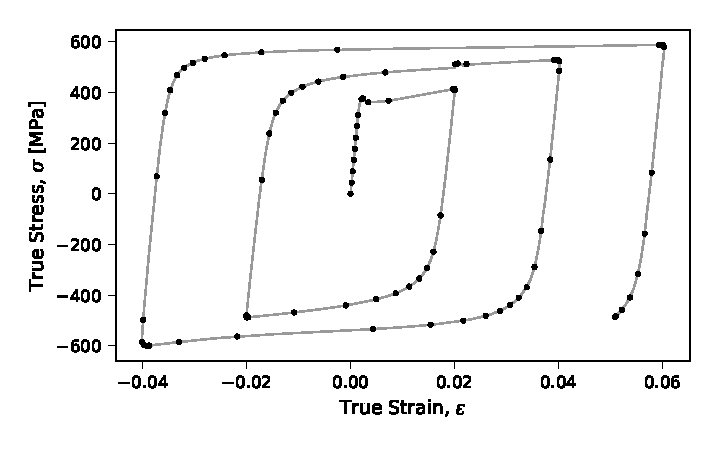
\includegraphics{HEM320_C_LP8_inds.pdf}
    \caption{Sampled points in LP8 from the HEM320 web dataset. Line = test data, dots = sampled points.}
    \label{fig:hem320-lp8-results}
\end{figure}

\section{Remarks}

\subsection{Different distance measures}

As outlined, a challenge in the max deviation downsampler is the difference in units between stress and strain.
I propose to re-scale the stress-strain data to then use a basic 2-norm when computing the perpendicular distance.
Two options that could be used rather than rescaling the data are:
\begin{enumerate}
    \item use the angle between the line and each point,
    \item use the norm induced by an alternative inner product: $\norm{d_k}_S = \sqrt{d_k \cdot S \cdot d_k}$, and
    \item use an energy criterion.
\end{enumerate}

The first option is similar to the maximum perpendicular distance, but more sensitive to noise.
This is because of the small angle rule, $\sin \theta \approx \theta$, and the perpendicular distance is $\norm{v}_2 \sin \theta$, where $v = x_k - x_i$.
If $\norm{v}_2$ is small, the angle can have a large variation (i.e., in the case of high frequency noise), however, the perpendicular distance remains small.

In the second option, Algorithm~\ref{alg:max-dev-downsampler} remains essential the same except for how $d_k$ is computed.
To use a matrix-vector notation:
\begin{equation*}
    d_k = \begin{bmatrix}
        d_{\varepsilon,k} \\
        d_{\sigma,k}
    \end{bmatrix}, \quad
    S = \begin{bmatrix}
        \frac{1}{(\max \varepsilon - \min \varepsilon)^2} & 0 \\
        0 & \frac{1}{(\max \sigma - \min \sigma)^2}
    \end{bmatrix},
\end{equation*}
where the values of $S$ would in this case give a similar effect to the scaling that I already use.
Other options for $S$ could be selected.
Essentially, we compute a scaled distance rather than scale the data itself.
This method would require a selection of tolerance $\epsilon$ and sample $j-1$ based on the same criterion.

In the third option, the perpendicular distance criterion is replaced by the energy bounded by the polygon.
In this case, instead of $d_k$'s we compute
\begin{equation*}
    e = \int_{\varepsilon_i}^{\varepsilon_j} (\sigma - l_\sigma) \dd \varepsilon,
\end{equation*}
where $l_\sigma$ represents the stress signal of the line between $x_i$ and $x_j$.
If the stress-strain graph is nearly straight, then $(\sigma - l_\sigma) \approx 0$.
The point $j-1$ would be sampled if $e > \epsilon$.

The benefits of the second method are that it does not require any scaling of the data and the error is closely related to the calibration problem.
However, the link between the energy, $e$, and the curvature in the stress-strain graph is less clear, making it more difficult to reason about an appropriate tolerance.
Everything considered, a tolerance still needs to be selected regardless of the method.
I went with the data scaling option because, in my opinion, the link between the algorithm and the geometric interpretation of curvature is most clear.

\subsection{More than two dimensions}

This document assumes two-dimensional data parametrized as a function of time, i.e., $x(t) \in \mathcal{D} \times \mathcal{T}$, where $\mathcal{D} \subset \mathbb{R}^n$ and $n$ is the dimension of the data ($n = 2$ in our case---uniaxial stress/strain), and $t \in \mathcal{T}$ is the time.
Algorithm~\ref{alg:overall-summary} can easily be extended to $n > 2$ by preserving curvature in each considered data pair.
The same procedure can then be used with an appropriate tolerance, $\epsilon$, and an appropriate scaling procedure by sampling a point anytime the tolerance is exceeded by one of the pairs.
Considering higher dimensions may be useful, for instance:
\begin{itemize}
    \item when downsampling temperature and stress-strain data together (can preserve curvature in both temperature-strain and stress-stress), and
    \item when downsampling data considering multiple components of the stress-strain tensor (e.g., multiaxial material tests).
\end{itemize}


\end{document}
